% !TEX program = pdflatex
% !BIB program  = biber
\documentclass[11pt, a4paper]{article}

%% ── Packages ────────────────────────────────────────────────────────────────
\usepackage[margin=1in]{geometry}
\usepackage{amsmath, amssymb, amsthm}
\usepackage{mathtools}          % \coloneqq, dcases, etc.
\usepackage{bm}                 % bold math
\usepackage{graphicx}
\usepackage{booktabs}           % professional tables
\usepackage{array}
\usepackage[hidelinks]{hyperref}
\usepackage[noabbrev, capitalise]{cleveref}
\usepackage[style=numeric, backend=biber, sorting=none]{biblatex}
\addbibresource{steering.bib}

%% ── Theorem-like environments ───────────────────────────────────────────────
\newtheorem{remark}{Remark}

%% ── Notation shorthands ─────────────────────────────────────────────────────
\newcommand{\kh}{\kappa_{\mathrm{heading}}}
\newcommand{\kg}{\kappa_{\mathrm{goal}}}
\newcommand{\Dp}{\Delta_{\mathrm{PFL3}}}
\newcommand{\sech}{\operatorname{sech}}

%% ─────────────────────────────────────────────────────────────────────────────
\title{\textit{Drosophila} Dual-Goal Steering Dynamics}
\author{Zhiyu Tian \and Yuqi Lin}
\date{May 12, 2026}
% ─────────────────────────────────────────────────────────────────────────────

\begin{document}
\maketitle

% ─────────────────────────────────────────────────────────────────────────────
\section{Introduction}
\label{sec:intro}
% ─────────────────────────────────────────────────────────────────────────────

Goal-directed navigation requires transforming allocentric spatial
representations into egocentric motor commands.  In \textit{Drosophila}, the
central complex implements this transformation through a well-characterised
circuit connecting the head direction system to descending motor neurons
\cite{westeinde2024}.  Three PFL neuron populations --- PFL3R, PFL3L, and PFL2
--- receive shifted copies of the head direction vector (phase shifts of
$+67.5°$, $-67.5°$, and $180°$ respectively) and compare these with a goal
vector represented in the fan-shaped body.  Each cell sums its heading input
with the goal input, passes the sum through a nonlinearity, and projects onto
the descending neurons DNa02 and DNa03 that ultimately drive steering.  The
full circuit, as characterised by Westeinde et al.\ \cite{westeinde2024},
implements a model of the steering system where the steering drive $U(\theta)$
is given by
%
\begin{equation}
\label{eq:steering}
\begin{aligned}
U(\theta) &=
  f\Bigl(
    \textstyle\sum g_{\mathrm{PFL3L}}
    + W_{\mathrm{DNa03}} \cdot
      f\bigl(\textstyle\sum g_{\mathrm{PFL3L}}
               + \textstyle\sum g_{\mathrm{PFL2L}}\bigr)
  \Bigr) \\[4pt]
&\quad -
  f\Bigl(
    \textstyle\sum g_{\mathrm{PFL3R}}
    + W_{\mathrm{DNa03}} \cdot
      f\bigl(\textstyle\sum g_{\mathrm{PFL3R}}
               + \textstyle\sum g_{\mathrm{PFL2R}}\bigr)
  \Bigr).
\end{aligned}
\end{equation}
%
This biological circuit-based model contains a direct pathway
(PFL3 $\to$ DNa02) with an indirect pathway (PFL3, PFL2 $\to$ DNa03 $\to$
DNa02) in which PFL2 cells provide adaptive gain control.  The resulting
rotational velocity $\dot\theta \propto U(\theta)$ varies sinusoidally with
directional error and produces a single stable fixed point at the goal.

This elegant architecture raises a natural question: \textbf{what happens when the fly
must navigate in the face of two simultaneous or competing goals?}  This project
investigates how the nonlinear structure of the PFL circuit, upon receiving two
simultaneous goal headings, can generate a double-well potential in heading
space, and derives conditions under which the resulting dynamics approximate the
forced Duffing oscillator --- a canonical model for chaos and complex
oscillations in nonlinear systems \cite{guckenheimer1983}.

To do so, in \cref{sec:derivation} we (i) extend the goal representation in
\cref{eq:steering} to a sum of two von Mises bumps at $\pm\delta$, modelling
two simultaneously presented goals; (ii) specialise the per-cell nonlinearity
to $f(x) = x^2$, which permits an exact closed-form evaluation of the
population integrals; and (iii) consider the simplified circuit in which PFL2
input is removed.  Under these assumptions, the steering signal
$U(\theta, \delta)$ can be derived analytically.  A local Taylor expansion of
$U(\theta, \delta)$ around $\theta = 0$, truncated at cubic order, produces
$\dot\theta \approx A(\delta,\kappa)\,\theta - B(\delta,\kappa)\,\theta^3$, the
right-hand side of a Duffing oscillator.

With the reduced system in hand, \cref{sec:bifurcation} establishes that this
system undergoes a supercritical pitchfork bifurcation, promotes the dynamics to
second order by adding inertia and damping, examines the resulting phase portrait,
and identifies its differences from the system before truncation.  Finally,
\cref{sec:chaos} characterises the onset of chaos under periodic forcing using
Melnikov's method and verifies the prediction numerically.

The Duffing reduction therefore serves as both a tractable analytical model of
the \textit{Drosophila} dual-goal steering dynamics and a useful diagnostic of
where neural-circuit dynamics share features with this well-characterised
nonlinear system.  The validity of the local reduction, and where it breaks down
in the full $S^1$ phase space, is a recurring theme throughout the report.


% ─────────────────────────────────────────────────────────────────────────────
\section{Derivation of the Reduced System}
\label{sec:derivation}
% ─────────────────────────────────────────────────────────────────────────────

\subsection{Analytical Form of the Steering Drive}
\label{sec:bessel}

Taking a reference frame in which the two goals
$\theta_{\mathrm{goal}}^{(0)}$ and $\theta_{\mathrm{goal}}^{(1)}$ are located
at $+\delta$ and $-\delta$ respectively, the von Mises bump representation of a
goal neuron with preferred direction $\phi$ is
%
\begin{equation}
\label{eq:goal-bump}
g_{\mathrm{goal}}(\phi, \delta)
  = \exp\bigl(\kg\cos(\delta - \phi)\bigr)
  + \exp\bigl(\kg\cos(-\delta - \phi)\bigr).
\tag{1}
\end{equation}
%
Similarly, a heading neuron with preference $\phi$ firing to the current heading
$\theta$ is
%
\begin{equation}
\label{eq:heading-bump}
g_{\mathrm{heading}}(\phi, \theta)
  = \exp\bigl(\kh\cos(\theta - \phi)\bigr).
\tag{2}
\end{equation}
%
Each PFL cell with goal preference $\phi$ receives a direct synaptic connection
from the associated goal neuron, and a connection from a heading neuron tuned
$\Dp$ away from $\phi$.  Taking the PFL3L subpopulation as the representative
example, the total drive to a PFL3L neuron with preference $\phi$ and the
resulting activity after the nonlinearity $f$ are
%
\begin{equation}
\label{eq:pfl3-drive}
\begin{aligned}
h_{\mathrm{PFL3L}}(\theta, \phi, \delta)
  &= S \cdot g_{\mathrm{heading}}(\phi - \Dp, \theta)
   + A \cdot g_{\mathrm{goal}}(\phi, \delta) \\
  &= S \cdot \exp\bigl(\kh\cos(\theta - (\phi - \Dp))\bigr) \notag\\
   &\quad+ A \cdot \bigl(
       \exp\bigl(\kg\cos(\delta - \phi)\bigr)
     + \exp\bigl(\kg\cos(-\delta - \phi)\bigr)
   \bigr), \\[4pt]
g_{\mathrm{PFL3L}}(\theta, \phi, \delta)
  &= f\bigl(h_{\mathrm{PFL3L}}(\theta, \phi, \delta)\bigr).
\end{aligned}
\tag{3}
\end{equation}
%
Because the downstream neurons DNa02 and DNa03 effectively integrate inputs
from all neurons in each population, the relevant quantity is the population
activity obtained by integrating \cref{eq:pfl3-drive} over all preferred
directions $\phi$:
%
\begin{equation}
\label{eq:pop-activity}
G_{\mathrm{PFL3L}}(\theta, \delta)
  = \int_{-\pi}^{\pi} g_{\mathrm{PFL3L}}(\theta, \phi, \delta)\,d\phi
  = \int_{-\pi}^{\pi} f\bigl(h_{\mathrm{PFL3L}}(\theta, \phi, \delta)\bigr)\,d\phi.
\tag{4}
\end{equation}

We choose the quadratic nonlinearity $f(x) = x^2$, a precedented choice in
computational neuroscience that allows conjunctive tuning for heading and goal
states at the level of PFL3 neurons \cite{hennequin2018}, and crucially
generates differences between the L and R populations after integration.
Expanding the square,
%
\begin{equation}
\label{eq:G-expanded}
\begin{aligned}
G_{\mathrm{PFL3L}}(\theta, \delta)
  &= \int_{-\pi}^{\pi} h_{\mathrm{PFL3L}}(\theta, \phi, \delta)^2\,d\phi \\
  &= \int_{-\pi}^{\pi}
     \Bigl[
       S^2 \cdot g_{\mathrm{heading}}(\phi - \Dp,\theta)^2
     + A^2 \cdot g_{\mathrm{goal}}(\phi,\delta)^2\notag\\
  &\quad+ 2SA \cdot g_{\mathrm{heading}}(\phi - \Dp,\theta)
             \cdot g_{\mathrm{goal}}(\phi,\delta)
     \Bigr] d\phi.
\end{aligned}
\tag{5}
\end{equation}
%
Because $\int_{-\pi}^{\pi} g_{\mathrm{heading}}(\phi - \Dp, \theta)^2\,d\phi
= \int_{-\pi}^{\pi} g_{\mathrm{heading}}(\phi + \Dp, \theta)^2\,d\phi$, the
purely heading-squared and purely goal-squared terms cancel in the
left-minus-right difference, giving
%
\begin{equation}
\label{eq:diff-pop}
\begin{aligned}
G_{\mathrm{PFL3L}} - G_{\mathrm{PFL3R}}
  &= 2SA \int_{-\pi}^{\pi}
     \bigl(
       g_{\mathrm{heading}}(\phi - \Dp, \theta)
     - g_{\mathrm{heading}}(\phi + \Dp, \theta)
     \bigr)
     g_{\mathrm{goal}}(\phi, \delta)\,d\phi \\
  &= 2SA \int_{-\pi}^{\pi}
     \bigl(
       e^{\kh\cos(\theta - (\phi - \Dp))}
     - e^{\kh\cos(\theta - (\phi + \Dp))}
     \bigr)\notag\\
     &\quad\cdot\bigl(
       e^{\kg\cos(\delta - \phi)}
     + e^{\kg\cos(-\delta - \phi)}
     \bigr)d\phi.
\end{aligned}
\tag{6}
\end{equation}
%
Defining $\xi_\phi(a, b) \colon S^1 \times S^1 \to \mathbb{R}$
by $\xi_\phi(a,b) \coloneqq \exp\bigl(
  \kh\cos(a - \phi) + \kg\cos(b - \phi)\bigr)$, \cref{eq:diff-pop} becomes
%
\begin{equation}
\label{eq:xi-form}
\begin{aligned}
G_{\mathrm{PFL3L}} - G_{\mathrm{PFL3R}}
  = 2SA \int_{-\pi}^{\pi} \bigl(
    &\xi_\phi(\theta + \Dp,\; \delta)
   + \xi_\phi(\theta + \Dp,\; -\delta) \\
   -&\xi_\phi(\theta - \Dp,\; \delta)
   - \xi_\phi(\theta - \Dp,\; -\delta)
  \bigr) d\phi.
\end{aligned}
\tag{7}
\end{equation}

The key identity is the phasor-sum of two cosines with the same argument
variable $\phi$:
%
\begin{equation}
\label{eq:phasor}
\kh\cos(\phi - a) + \kg\cos(\phi - b) = \kappa(a, b)\cos(\phi - \mu(a,b)),
\end{equation}
%
where the effective concentration and phase are
%
\begin{equation}
\label{eq:kappa}
\kappa(a, b)
  = \sqrt{\kh^2 + \kg^2 + 2\kh\kg\cos(a - b)},
\end{equation}
%
\begin{equation}
\label{eq:mu}
\mu(a, b)
  = \operatorname{atan2}\bigl(
      \kh\sin a + \kg\sin b,\;
      \kh\cos a + \kg\cos b
    \bigr).
\end{equation}
%
The phase $\mu$ depends on $a$ and $b$ but drops out upon integration over the
full period in $\phi$, since $\int_{-\pi}^{\pi} \exp(\kappa\cos(\phi -
\mu))\,d\phi = 2\pi I_0(\kappa)$ for any $\mu$, by translation invariance of
the uniform measure on $S^1$ (here $I_0$ is the modified Bessel function of the
first kind of order zero).  Accordingly,
%
\begin{equation}
\label{eq:bessel-integral}
\int_{-\pi}^{\pi} \xi_\phi(a, b)\,d\phi
  = \int_{-\pi}^{\pi} \exp\bigl(\kappa(a,b)\cos(\phi - \mu(a,b))\bigr)\,d\phi
  = 2\pi I_0\bigl(\kappa(a, b)\bigr).
\tag{8}
\end{equation}
%
Applying this to each of the four terms in \cref{eq:xi-form} yields the
closed-form steering drive:
%
\begin{equation}
\label{eq:G-closed}
\begin{aligned}
G_{\mathrm{PFL3L}} - G_{\mathrm{PFL3R}}
  = 4\pi SA \Bigl(
    &I_0\bigl(\kappa(\theta + \Dp,\; \delta)\bigr)
   + I_0\bigl(\kappa(\theta + \Dp,\; -\delta)\bigr) \\
   -&I_0\bigl(\kappa(\theta - \Dp,\; \delta)\bigr)
   - I_0\bigl(\kappa(\theta - \Dp,\; -\delta)\bigr)
  \Bigr).
\end{aligned}
\tag{9}
\end{equation}
%
In the simplified circuit without PFL2 input --- in which DNa02 and DNa03
simply sum the PFL3L and PFL3R population activities, respectively --- the
steering drive is
%
\begin{equation}
\label{eq:U-bessel}
U(\theta, \delta) = G_{\mathrm{PFL3L}}(\theta,\delta) - G_{\mathrm{PFL3R}}(\theta,\delta).
\tag{10}
\end{equation}
%
This expression will be referred to as the \emph{Bessel model} throughout.

Numerical evaluation of the Bessel model, the discrete PFL3 model with 12
neurons on each side (matching the biological circuit), and the full circuit
model including PFL2 yield nearly identical $U(\theta)$ profiles
(\cref{fig:U-profiles}), supporting the validity of these simplifications.  All
subsequent analysis employs the PFL3-only circuit, using the 12-neuron discrete
model as the ground-truth comparison.

\begin{figure}[htbp]
  \centering
  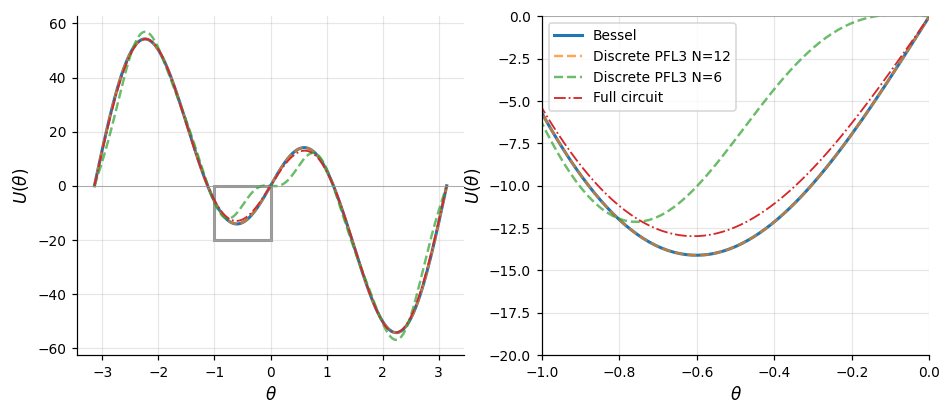
\includegraphics[width=0.85\textwidth]{figures/fig1.png}
  \caption{Steering drive $U(\theta)$ from different circuit models.}
  \label{fig:U-profiles}
\end{figure}


% ─────────────────────────────────────────────────────────────────────────────
\subsection{Taylor Expansion of the Steering Drive}
\label{sec:taylor}

\subsubsection{Symmetry of \texorpdfstring{$U(\theta, \delta)$}{U(theta,delta)}}
\label{sec:symmetry}

Before computing the Taylor expansion, we record two symmetry properties that
simplify the derivatives at $\theta = 0$.

\medskip
\noindent\textit{Property (a).} $\kappa(a, b)$ depends on $a, b$ only through
$\cos(a - b)$, which follows directly from \cref{eq:kappa}.

\medskip
\noindent\textit{Property (b).} $U$ is odd in $\theta$ at fixed $\delta$: apply
the substitution $\theta \to -\theta$ to the four arguments in \cref{eq:G-closed}
according to the following table.

\begin{center}
\begin{tabular}{ll}
\toprule
Original & After $\theta \to -\theta$ \\
\midrule
$\kappa(\theta + \Dp,\; \delta)$  & $\kappa(-\theta + \Dp,\; \delta)$ \\
$\kappa(\theta + \Dp,\; -\delta)$ & $\kappa(-\theta + \Dp,\; -\delta)$ \\
$\kappa(\theta - \Dp,\; \delta)$  & $\kappa(-\theta - \Dp,\; \delta)$ \\
$\kappa(\theta - \Dp,\; -\delta)$ & $\kappa(-\theta - \Dp,\; -\delta)$ \\
\bottomrule
\end{tabular}
\end{center}

Using property (a) --- $\kappa$ depends on its arguments only through their
cosine difference --- one verifies that $\kappa(-\theta + \Dp, \delta)
= \kappa(\theta - \Dp, -\delta)$, and similarly for the remaining three pairs.
Working through all four terms, the four arguments after $\theta \to -\theta$
are precisely the four original terms with their signs swapped, giving
%
\begin{equation}
\label{eq:U-odd}
U(-\theta, \delta) = -U(\theta, \delta).
\end{equation}
%
As corollaries: $U(0, \delta) = 0$ for all $\delta$, and all even-order
derivatives vanish at $\theta = 0$, i.e.\ $U^{(2k)}(0, \delta) = 0$ for
$k = 0, 1, 2, \ldots$

\subsubsection{Taylor expansion around \texorpdfstring{$\theta = 0$}{theta=0}}
\label{sec:taylor-expansion}

Expanding $U(\theta, \delta)$ around $\theta = 0$,
%
\begin{equation}
\label{eq:taylor-full}
U(\theta, \delta)
  = U(0,\delta)
  + U'(0,\delta)\,\theta
  + \tfrac{1}{2}U''(0,\delta)\,\theta^2
  + \tfrac{1}{6}U'''(0,\delta)\,\theta^3
  + O(\theta^4).
\tag{11}
\end{equation}
%
By \cref{sec:symmetry},
%
\begin{equation}
\label{eq:even-vanish}
U(0, \delta) = 0, \qquad U''(0, \delta) = 0.
\tag{12}
\end{equation}
%
Only the odd-order terms survive, yielding the Duffing-type truncation
%
\begin{equation}
\label{eq:duffing-form-firstorder}
U(\theta, \delta) \approx U'(0,\delta)\,\theta
                        + \tfrac{1}{6}U'''(0,\delta)\,\theta^3
                        + O(\theta^5).
\end{equation}

\subsubsection{First-order coefficient}
\label{sec:A-coeff}

Define $K(\theta; a, b) \coloneqq \kappa(\theta + a, b)$.  By the chain rule
and the identity $I_0'(x) = I_1(x)$,
%
\begin{equation}
\label{eq:dI0-chain}
\frac{d}{d\theta} I_0\bigl(K(\theta; a,b)\bigr)
  = I_1(K) \cdot \frac{dK}{d\theta}.
\tag{13a}
\end{equation}
%
From $K^2 = \kh^2 + \kg^2 + 2\kh\kg\cos(\theta + a - b)$, differentiating
implicitly gives $2K\,dK/d\theta = -2\kh\kg\sin(\theta + a - b)$, hence
%
\begin{equation}
\frac{dK}{d\theta}
  = -\frac{\kh\kg\sin(\theta + a - b)}{K(\theta; a, b)}.
\tag{13b}
\end{equation}
%
Combining,
%
\begin{equation}
\frac{d}{d\theta} I_0\bigl(K(\theta; a,b)\bigr)
  = -I_1(K)\cdot\frac{\kh\kg\sin(\theta + a - b)}{K}.
\tag{13c}
\end{equation}
%
Applying this to each of the four terms in \cref{eq:G-closed} and evaluating at
$\theta = 0$, then using property (a) to pair the four terms into two, yields
%
\begin{equation}
\label{eq:Uprime}
\boxed{
U'(0, \delta)
  = -8\pi SA\,\kh\kg
    \left[
      \frac{I_1(\kappa(\Dp, \delta))}{\kappa(\Dp, \delta)}
      \sin(\Dp - \delta)
    + \frac{I_1(\kappa(\Dp, -\delta))}{\kappa(\Dp, -\delta)}
      \sin(\Dp + \delta)
    \right].
}
\tag{14}
\end{equation}

\subsubsection{Third-order coefficient}
\label{sec:B-coeff}

We require $d^3 I_0(K)/d\theta^3\big|_{\theta=0}$.  Set
\begin{equation}
C(\theta) \coloneqq \kh\kg\cos(\theta + a - b),
\qquad
\mathcal{S}(\theta) \coloneqq \kh\kg\sin(\theta + a - b),
\end{equation}
so that $K^2 = \kh^2 + \kg^2 + 2C$.  Successive differentiation gives
%
\begin{align}
K'   &= -\frac{\mathcal{S}}{K}, \notag\\
K''  &= -\frac{C}{K} - \frac{\mathcal{S}^2}{K^3}, \notag\\
K''' &= \frac{\mathcal{S}}{K} - \frac{3\mathcal{S}C}{K^3} - \frac{3\mathcal{S}^3}{K^5}.
\label{eq:Kderivs}
\end{align}
%
For the Bessel side, the recurrences $I_0' = I_1$, $I_1' = \tfrac{1}{2}(I_0 +
I_2)$, and $I_1'' = \tfrac{1}{4}(3I_1 + I_3)$ give
%
\begin{align}
I_0'   &= I_1, \notag\\
I_0''  &= \tfrac{1}{2}\bigl[I_0(x) + I_2(x)\bigr], \notag\\
I_0''' &= \tfrac{1}{4}\bigl[3I_1(x) + I_3(x)\bigr].
\label{eq:Iderivs}
\end{align}
%
Applying the chain rule three times:
%
\begin{equation}
\label{eq:d3I0}
\begin{aligned}
\frac{d^3}{d\theta^3} I_0(K)
  &= I_0'''(K)\,(K')^3
   + 3\,I_0''(K)\,K'\,K''
   + I_0'(K)\,K''' \\
  &= \frac{3I_1(K)+I_3(K)}{4}
     \cdot\left(-\frac{\mathcal{S}^3}{K^3}\right) \\
  &\quad
   + 3 \cdot \frac{I_0(K)+I_2(K)}{2}
     \cdot\left(\frac{\mathcal{S}C}{K^2} + \frac{\mathcal{S}^3}{K^4}\right) \\
  &\quad
   + I_1(K)
     \cdot\left(\frac{\mathcal{S}}{K} - \frac{3C\mathcal{S}}{K^3}
                - \frac{3\mathcal{S}^3}{K^5}\right).
\end{aligned}
\end{equation}
%
With $d^3 I_0(K)/d\theta^3$ in hand, the third-order coefficient of $U$ is the
signed sum over the four arguments of \cref{eq:G-closed}:
%
\begin{equation}
\label{eq:U-triple-prime}
U'''(0, \delta)
  = 4\pi SA
    \sum_{(a,b) \in \mathcal{P}}
    \sigma(a) \cdot
    \frac{d^3}{d\theta^3} I_0\bigl(K(\theta; a, b)\bigr)\Bigr|_{\theta=0},
\tag{16}
\end{equation}
%
where $\mathcal{P} = \{(\Dp,\delta),\, (\Dp,-\delta),\,
(-\Dp,\delta),\, (-\Dp,-\delta)\}$ and $\sigma(a) = +1$ for $a = +\Dp$,
$-1$ for $a = -\Dp$.  Using property (a) to pair the four terms gives
%
\begin{equation}
\label{eq:Utriprime-box}
\boxed{
U'''(0, \delta)
  = 8\pi SA\,\kh\kg
    \bigl[
      \sin(\Dp - \delta)\cdot D(\kappa_-, C_-, \mathcal{S}_-)
    + \sin(\Dp + \delta)\cdot D(\kappa_+, C_+, \mathcal{S}_+)
    \bigr],
}
\tag{17}
\end{equation}
%
where
%
\begin{equation}
\label{eq:D-def}
\begin{aligned}
D(K,C,\mathcal{S})
  &= \frac{1}{K}
     \Biggl[
       I_1(K)\left(1 - \frac{3C}{K^2} - \frac{3\mathcal{S}^2}{K^4}\right)
     + \frac{3\bigl(I_0(K) + I_2(K)\bigr)}{2}
       \left(\frac{C}{K} + \frac{\mathcal{S}^2}{K^3}\right)
     - \frac{3I_1(K) + I_3(K)}{4}\cdot\frac{\mathcal{S}^2}{K^2}
     \Biggr],
\end{aligned}
\end{equation}
%
and
%
\begin{align}
\kappa_- &\equiv \kappa(\Dp, \delta)
  = \sqrt{\kh^2 + \kg^2 + 2\kh\kg\cos(\Dp - \delta)}, \notag\\
\kappa_+ &\equiv \kappa(\Dp, -\delta)
  = \sqrt{\kh^2 + \kg^2 + 2\kh\kg\cos(\Dp + \delta)}, \notag\\
C_- &\equiv \kh\kg\cos(\Dp - \delta), \quad
C_+ \equiv \kh\kg\cos(\Dp + \delta), \notag\\
\mathcal{S}_- &\equiv \kh\kg\sin(\Dp - \delta), \quad
\mathcal{S}_+ \equiv \kh\kg\sin(\Dp + \delta).
\label{eq:kappa-pm}
\end{align}

\subsubsection{Local cubic expansion}
\label{sec:cubic}

Combining \cref{sec:A-coeff,sec:B-coeff}, the local expansion of the steering
drive is
%
\begin{equation}
\label{eq:cubic-ode}
\dot{\theta} = U(\theta, \delta)
  \approx A(\delta)\,\theta - B(\delta)\,\theta^3 + O(\theta^5),
\tag{18}
\end{equation}
%
with
%
\begin{equation}
\label{eq:AB-def}
A(\delta) \equiv U'(0, \delta),
\qquad
B(\delta) \equiv -\tfrac{1}{6}\,U'''(0, \delta),
\end{equation}
%
matching the conventional sign convention of the Duffing oscillator.


% ─────────────────────────────────────────────────────────────────────────────
\subsection{Body Mechanics and Second-Order Dynamics}
\label{sec:body}
% ─────────────────────────────────────────────────────────────────────────────

Model the fly as a rigid body with rotational inertia $I$ and rotational drag
$\gamma$.  The reduction of \cref{sec:bessel,sec:cubic} yields a first-order
equation in which the circuit output is interpreted as a direct angular-velocity
command --- the overdamped limit of the heading dynamics.  Restoring the inertia
and interpreting $U(\theta, \delta)$ as a \textbf{torque command}, Newton's second law
gives
%
\begin{equation}
\label{eq:newton}
I\ddot{\theta} + \gamma\dot{\theta} = U(\theta,\delta).
\tag{19}
\end{equation}
%
The first-order model is recovered as the overdamped limit $I \to 0$: when
inertia is negligible relative to drag, $\ddot\theta$ drops out and one recovers
$\gamma\dot\theta = U$.  We stress that this is a modelling reinterpretation:
the constants $I$ and $\gamma$ enter as phenomenological parameters describing
body dynamics rather than being derived from the circuit.  (An alternative
reading is that $I$ represents an effective inertia arising from circuit and
motor lags.)

Substituting the local cubic expansion of \cref{sec:cubic} into
\cref{eq:newton},
%
\begin{equation}
\label{eq:duffing-unforced}
I\ddot\theta + \gamma\dot\theta = A(\delta,\kappa)\,\theta - B(\delta,\kappa)\,\theta^3,
\tag{20}
\end{equation}
%
which is the canonical \textbf{unforced double-well Duffing oscillator}.


% ─────────────────────────────────────────────────────────────────────────────
\section{Equilibrium Structure and Bifurcation Analysis}
\label{sec:bifurcation}
% ─────────────────────────────────────────────────────────────────────────────

\subsection{Supercritical Pitchfork Bifurcation and Double-Well Criterion}
\label{sec:pitchfork}

The first-order system derived from the circuit model shares equilibrium
structure with the unforced double-well Duffing oscillator \eqref{eq:duffing-unforced}:
equilibria occur at $\theta = 0$ and $\theta = \pm\sqrt{A/B}$ whenever
$A/B > 0$.

Linearising at the origin, $\dot\theta = A\theta$, shows that the fixed point at
$\theta = 0$ is unstable --- i.e.\ a double-well structure exists --- if and
only if $A(\delta,\kappa) = U'(0,\delta) > 0$.  Substituting from \cref{eq:Uprime},
the bifurcation curve $A(\delta) = 0$ is
%
\begin{equation}
\label{eq:bif-curve}
-8\pi SA\,\kh\kg
\left[
  \frac{I_1(\kappa(\Dp, \delta))}{\kappa(\Dp, \delta)} \sin(\Dp - \delta)
+ \frac{I_1(\kappa(\Dp, -\delta))}{\kappa(\Dp, -\delta)} \sin(\Dp + \delta)
\right] = 0.
\end{equation}
%
When in addition $B(\delta,\kappa) > 0$ (i.e.\ $U'''(0,\delta) < 0$), two new
equilibria emerge at $\theta = \pm\sqrt{A/B}$, giving the double-well structure.
From \cref{eq:Utriprime-box}, the condition for a supercritical pitchfork is
%
\begin{equation}
\label{eq:supercritical}
8\pi SA\,\kh\kg
\bigl[
  \sin(\Dp - \delta)\cdot D(\kappa_-, C_-, \mathcal{S}_-)
+ \sin(\Dp + \delta)\cdot D(\kappa_+, C_+, \mathcal{S}_+)
\bigr] < 0.
\end{equation}
%
These are transcendental equations in $(\delta, \kh, \kg)$ at fixed $\Dp =
67.5°$.  Setting $\kh = \kg \equiv \kappa$ collapses the parameter space to
$(\delta, \kappa)$.  Numerical solutions yield the bifurcation diagram shown in
\cref{fig:bifurcation}.

\begin{figure}[htbp]
  \centering
  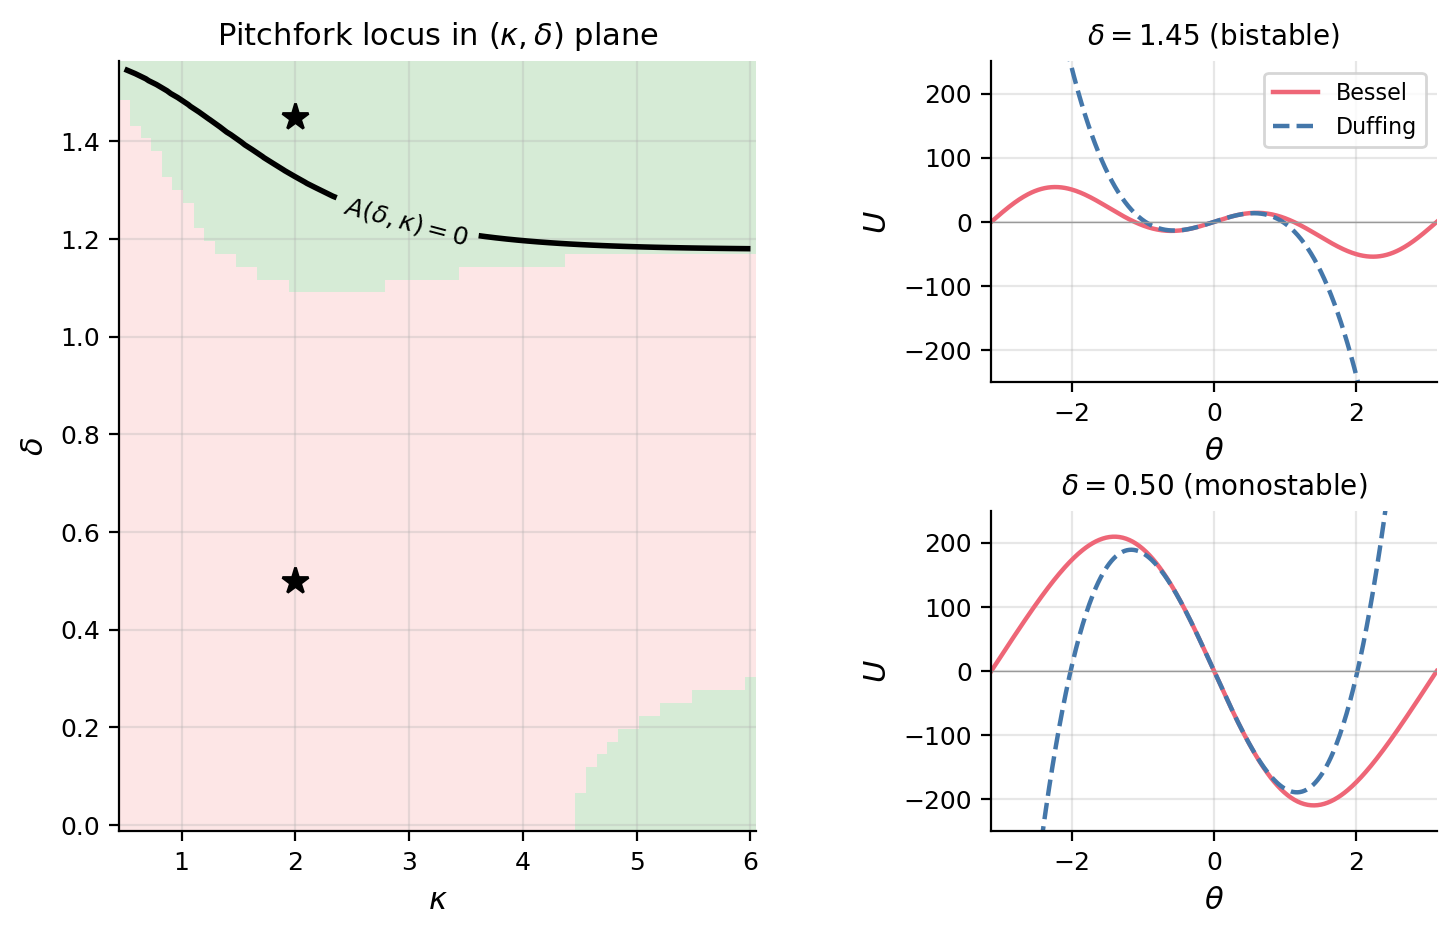
\includegraphics[width=0.85\textwidth]{figures/fig2.png}
  \caption{Pitchfork bifurcation in $(\kappa, \delta)$ parameter space.  Left:
  the black curve marks the pitchfork bifurcation, where the origin changes
  stability.  Above the curve, $A > 0$ and the origin is unstable; below, $A <
  0$ and the origin is the unique stable fixed point.  Green shading indicates
  $B(\delta,\kappa) > 0$ (supercritical pitchfork); red shading indicates $B <
  0$.  Right: the exact steering drive $U(\theta)$ (red, Bessel model) with its
  local Duffing truncation (blue dashed) at two sample parameter points.}
  \label{fig:bifurcation}
\end{figure}

The bifurcation boundary lies entirely within the region where $B(\delta,\kappa)
> 0$ (green shading), confirming that the pitchfork is supercritical everywhere:
the transition from monostable to bistable is smooth, with no jumps or
hysteresis.  The upper-right panel shows a sample point from the bistable region.
The local Duffing approximation is accurate near $\theta = 0$, capturing the
saddle and the two flanking stable equilibria; at large $\theta$ it diverges from
the exact Bessel model, which has additional zero-crossings near $\theta = \pm\pi$
corresponding to saddle points at the anti-midpoint of the two goals.  The
Duffing reduction is therefore reliable for small-amplitude dynamics, while
global features of the $S^1$ phase space require the full Bessel model.


% ─────────────────────────────────────────────────────────────────────────────
\subsection{Phase Portrait}
\label{sec:phase-portrait}
% ─────────────────────────────────────────────────────────────────────────────

To set up the chaos analysis in \cref{sec:chaos}, we first examine the full
phase space of the second-order system in its conservative limit ($\gamma = 0$).
With damping set to zero in \cref{eq:newton},
%
\begin{equation}
\label{eq:conservative}
I\ddot{\theta} = U(\theta,\delta).
\end{equation}
%
This system conserves the energy
%
\begin{equation}
\label{eq:energy}
H(\theta,\dot{\theta})
  = \tfrac{1}{2}I\dot{\theta}^2 + V(\theta),
\qquad
V(\theta) = -\int_0^{\theta} U(\theta',\delta)\,d\theta',
\tag{21}
\end{equation}
%
and trajectories lie on the level sets of $H$ in the phase plane
$(\theta,\dot\theta)$.  Equilibria are zeros of $U(\theta,\delta)$, with
stability determined by the sign of $V''(\theta)$.

\begin{figure}[htbp]
  \centering
  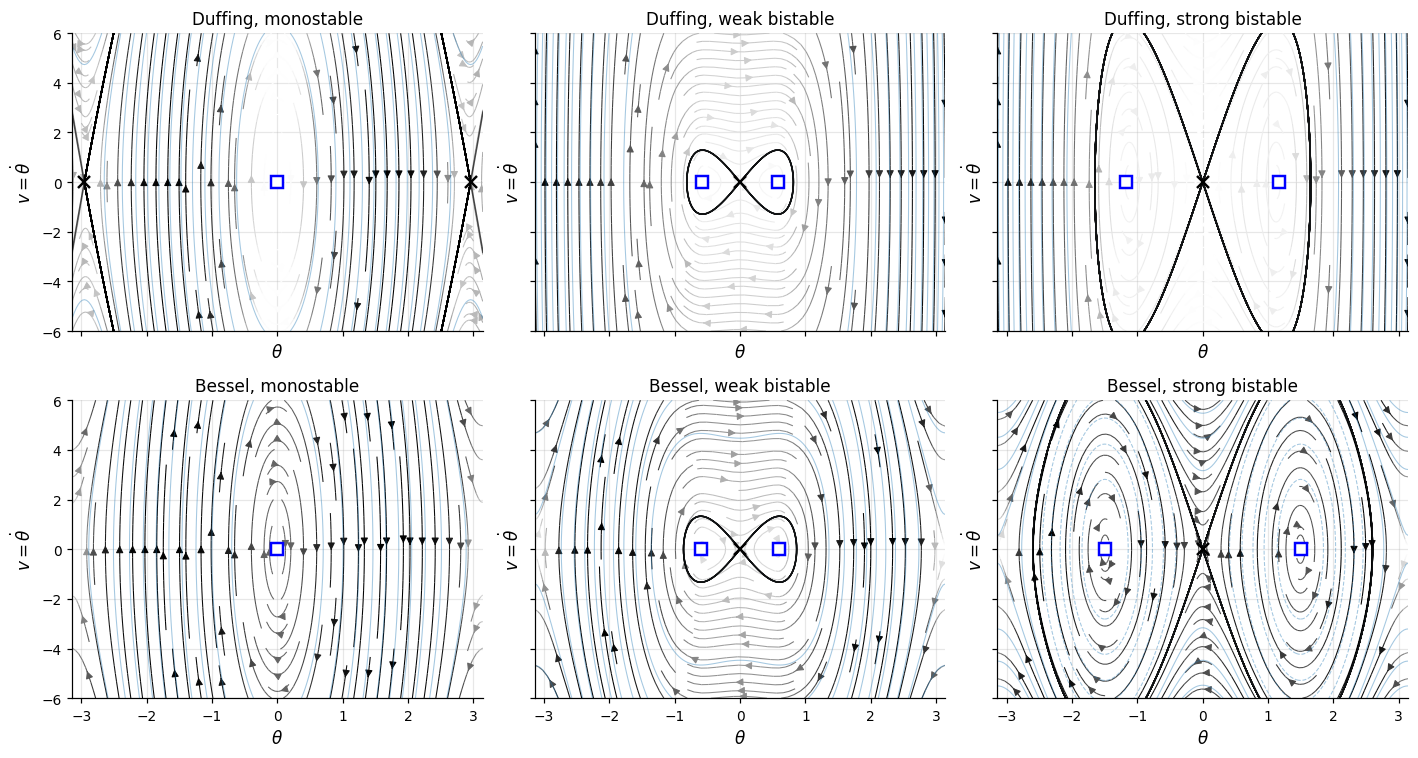
\includegraphics[width=\textwidth]{figures/fig3.png}
  \caption{Phase portrait with $\kg = \kh = 2$, $\delta \in \{1,\, 1.36,\,
  1.55\}$.  Top row: Duffing truncation.  Bottom row: exact Bessel model.
  Columns correspond to the monostable ($A < 0$), weakly bistable ($A$ slightly
  positive), and strongly bistable ($A > 0$) regimes of the pitchfork
  bifurcation curve.}
  \label{fig:phase-portrait}
\end{figure}

In the monostable case, both models exhibit a single centre at $\theta = 0$
surrounded by closed orbits corresponding to small-amplitude oscillations.  In
the weakly bistable case, crossing the pitchfork curve gives rise to the
classical figure-eight separatrix: two centres at $\theta_\pm = \pm\sqrt{A/B}$
flank a saddle at the origin, joined by a pair of homoclinic orbits bounding the
oscillatory motion.  The Duffing and Bessel portraits are nearly
indistinguishable in this regime, and we work here for the remainder of the
analysis.  In the strongly bistable regime, the two models diverge
geometrically: the Duffing truncation continues to predict a closed figure-eight,
while the exact Bessel system shows the saddle's stable and unstable manifolds
extending toward the secondary saddles near $\theta = \pm\pi$, which themselves are connected with heteroclinic orbits.  We return to this point in
\cref{sec:phase-slipping}.


% ─────────────────────────────────────────────────────────────────────────────
\subsection{The Homoclinic Orbit}
\label{sec:homoclinic}
% ─────────────────────────────────────────────────────────────────────────────

The unforced, undamped reduced system
$\ddot\theta = A\theta - B\theta^3$
with $A, B > 0$ is a planar Hamiltonian system with conserved energy
%
\begin{equation}
\label{eq:H-duffing}
H(\theta, \dot{\theta})
  = \tfrac{1}{2}\dot{\theta}^2 - \tfrac{1}{2}A\theta^2 + \tfrac{1}{4}B\theta^4.
\tag{22}
\end{equation}
%
The zero-energy level set $H = 0$ consists of two homoclinic loops joining the
saddle at the origin to itself.  Solving $\frac{1}{2}\dot\theta^2 =
\frac{1}{2}A\theta^2 - \frac{1}{4}B\theta^4$ on the right branch gives the
closed-form homoclinic orbit
%
\begin{equation}
\label{eq:homoclinic}
\boxed{
\theta_0(t)
  = \sqrt{\tfrac{2A}{B}}\,\sech(\sqrt{A}\,t),
\qquad
v_0(t)
  = -\sqrt{\tfrac{2A}{B}}\sqrt{A}\,\sech(\sqrt{A}\,t)\tanh(\sqrt{A}\,t).
}
\tag{23}
\end{equation}
%
This orbit reaches its apex $\theta_{\max} = \sqrt{2A/B}$ at $t = 0$ and
approaches the saddle exponentially at rate $\sqrt{A}$ as $t \to \pm\infty$.
The loop in the left half-plane is obtained by $\theta_0 \to -\theta_0$; their
union forms the figure-eight separatrix dividing the phase plane into the two
wells and the region of unbounded growth.


% ─────────────────────────────────────────────────────────────────────────────
\section{Chaotic Behaviour Under Periodic Forcing}
\label{sec:chaos}
% ─────────────────────────────────────────────────────────────────────────────

\subsection{Damped, Forced Duffing Oscillator}
\label{sec:forced}

We have established that the steering circuit reduced to its local cubic normal
form (\cref{eq:duffing-unforced}) is the unforced double-well Duffing oscillator,
and that the bistable regime is entered through a supercritical pitchfork in
$(\delta, \kappa)$ parameter space.  We now ask what happens when this system is
driven by periodic forcing.  The forced system reads
%
\begin{equation}
\label{eq:forced-duffing}
\ddot\theta + \gamma\dot\theta = U(\theta, \delta) + F\cos(\omega t),
\tag{24}
\end{equation}
%
where we have set $I = 1$ for notational economy (this fixes a time scale; all
reported frequencies are in units of $\sqrt{I^{-1}}$).  The forced Duffing
oscillator is the canonical example of a low-dimensional smooth system that
exhibits Smale horseshoe chaos for sufficiently strong forcing
\cite{guckenheimer1983}.  Our goals in this section are (i) to derive an
analytical condition on $(F, \omega, \gamma, \delta, \kappa)$ at which chaotic
dynamics first becomes possible in the reduced system, via Melnikov's method, and
(ii) to verify this condition numerically in both the reduced (Duffing) and Bessel
models.  In doing so, we characterise a second, qualitatively distinct chaotic
regime that emerges in the global $S^1$ system but is invisible to the local
Duffing reduction.


% ─────────────────────────────────────────────────────────────────────────────
\subsection{The Melnikov Criterion}
\label{sec:melnikov}
% ─────────────────────────────────────────────────────────────────────────────

Following \textcite{guckenheimer1983}, \S4.5, we cast \cref{eq:forced-duffing}
as an $O(\epsilon)$ perturbation of the Hamiltonian system \eqref{eq:H-duffing}:
%
\begin{equation}
\label{eq:perturbed-system}
\dot\theta = v,
\qquad
\dot v = U(\theta, \delta) + \epsilon\bigl[-\gamma v + F\cos\omega t\bigr].
\tag{25}
\end{equation}
%
We write $U(\theta,\delta)$ here for the local Duffing $A\theta - B\theta^3$,
but the derivation below extends to the full Bessel $U$ (exploited in
\cref{sec:numerical-melnikov}).  To leading order in $\epsilon$, the Melnikov
function $M(t_0)$ measures the signed distance between the stable and unstable
manifolds of the perturbed saddle --- now a hyperbolic periodic orbit of period
$2\pi/\omega$ in extended phase space --- at a fixed phase $\omega t_0$ of the
forcing cycle.  Simple zeros of $M(t_0)$ correspond to transverse manifold
intersections which, by the Smale--Birkhoff theorem, imply the existence of a
Smale horseshoe and hence chaotic dynamics \cite[Theorem~4.5.3]{guckenheimer1983}.

Writing the unperturbed flow as $\mathbf{f}(\mathbf{x}) = (v,\,U(\theta))^T$
and the perturbation as $\mathbf{g}(\mathbf{x}, t) = (0,\,-\gamma v +
F\cos\omega t)^T$, the Melnikov function is
\cite[\S4.5]{guckenheimer1983}
%
\begin{equation}
\label{eq:melnikov-def}
M(t_0)
  = \int_{-\infty}^{\infty}
    \mathbf{f}\bigl(\boldsymbol{\gamma}_0(\tau)\bigr)
    \wedge
    \mathbf{g}\bigl(\boldsymbol{\gamma}_0(\tau),\, \tau + t_0\bigr)
    \,d\tau,
\tag{26}
\end{equation}
%
where $\mathbf{f} \wedge \mathbf{g} \coloneqq f_1 g_2 - f_2 g_1$ is the scalar
wedge product in $\mathbb{R}^2$, and $\boldsymbol{\gamma}_0(\tau) =
(\theta_0(\tau), v_0(\tau))$ is the unperturbed homoclinic orbit.  Expanding the
wedge,
%
\begin{equation}
\label{eq:wedge-expand}
\mathbf{f} \wedge \mathbf{g}
  = v\bigl[-\gamma v + F\cos\omega t\bigr] - U(\theta)\cdot 0
  = -\gamma v^2 + Fv\cos\omega t.
\tag{27}
\end{equation}
%
The steering drive $U(\theta)$ drops out of the integrand entirely; it enters
only through its role in shaping the homoclinic orbit $\boldsymbol{\gamma}_0$.
The Melnikov formula becomes
%
\begin{equation}
\label{eq:melnikov-split}
M(t_0)
  = -\gamma\int_{-\infty}^{\infty} v_0(\tau)^2\,d\tau
  + F\int_{-\infty}^{\infty} v_0(\tau)\cos\omega(\tau + t_0)\,d\tau.
\tag{28}
\end{equation}
%
\textit{Damping integral.}  With $u = \sqrt{A}\,\tau$ and the elementary result
$\int_{-\infty}^{\infty} \sech^2 u\,\tanh^2 u\,du = 2/3$,
%
\begin{equation}
\label{eq:D-integral}
D \coloneqq \int_{-\infty}^{\infty} v_0(\tau)^2\,d\tau
  = \frac{2A^2}{B}\cdot\frac{1}{\sqrt{A}}\cdot\frac{2}{3}
  = \frac{4A^{3/2}}{3B}.
\tag{29}
\end{equation}
%
\textit{Forcing integral.}  Expanding $\cos\omega(\tau + t_0) = \cos\omega\tau
\cos\omega t_0 - \sin\omega\tau\sin\omega t_0$ and noting that $v_0(\tau)$ is
odd, the cosine piece integrates to zero, leaving
%
\begin{equation}
\label{eq:F-integral-setup}
\int_{-\infty}^{\infty} v_0(\tau)\cos\omega(\tau + t_0)\,d\tau
  = -\sin\omega t_0
    \int_{-\infty}^{\infty} v_0(\tau)\sin\omega\tau\,d\tau.
\end{equation}
%
Using the contour-integration identity, derived by summing residues at the poles
$\tau = i\pi(n + \tfrac{1}{2})/\alpha$ of $\sech$,
%
\begin{equation}
\label{eq:contour}
\int_{-\infty}^{\infty}
  \sech(\alpha\tau)\tanh(\alpha\tau)\sin\omega\tau\,d\tau
  = -\frac{\pi\omega}{\alpha^2}\sech\left(\frac{\pi\omega}{2\alpha}\right),
\end{equation}
%
with $\alpha = \sqrt{A}$,
%
\begin{equation}
\label{eq:forcing-integral}
\int_{-\infty}^{\infty} v_0(\tau)\sin\omega\tau\,d\tau
  = \pi\omega\sqrt{\frac{2}{B}}\;\sech\left(\frac{\pi\omega}{2\sqrt{A}}\right).
\tag{30}
\end{equation}
%
Combining \cref{eq:D-integral,eq:F-integral-setup,eq:forcing-integral},
%
\begin{equation}
\label{eq:melnikov-final}
\boxed{
M(t_0)
  = -\frac{4\gamma A^{3/2}}{3B}
  - F\pi\omega\sqrt{\frac{2}{B}}\;\sech\left(\frac{\pi\omega}{2\sqrt{A}}\right)
    \sin\omega t_0.
}
\tag{31}
\end{equation}
%
$M(t_0)$ has simple zeros if and only if the amplitude of the sinusoidal term
exceeds the damping bias, yielding the Melnikov threshold
%
\begin{equation}
\label{eq:Fcrit}
\boxed{
F_{\mathrm{crit}}(\omega)
  = \frac{4\gamma A}{3\pi\omega\sqrt{2B}}
    \cosh\left(\frac{\pi\omega}{2\sqrt{A}}\right).
}
\tag{32}
\end{equation}
%
Two features of \cref{eq:Fcrit} deserve emphasis.  First, $F_{\mathrm{crit}}
\to \infty$ as $\omega \to 0$ and as $\omega \to \infty$: both very-low-
and very-high-frequency forcing are inefficient at inducing chaos.  The threshold
is minimised at $\omega^* \approx 0.76\sqrt{A}$, obtained from
$\tanh(\pi\omega^*/2\sqrt{A}) = 2\sqrt{A}/(\pi\omega^*)$.  Second, the
dependence on the well structure enters only through $A$ and $B$, which in turn
depend non-trivially on $(\delta, \kappa, S, A_{\mathrm{syn}})$ via
\cref{eq:Uprime,eq:Utriprime-box}; \cref{eq:Fcrit} therefore implicitly maps the
chaos-onset surface into circuit parameter space.


% ─────────────────────────────────────────────────────────────────────────────
\subsection{Numerical Melnikov Analysis on the Bessel Homoclinic}
\label{sec:numerical-melnikov}
% ─────────────────────────────────────────────────────────────────────────────

The derivation of \cref{sec:melnikov} holds equally for the full Bessel system;
only the homoclinic orbit changes.  We exploit this to extend the Melnikov
prediction beyond the cubic truncation by evaluating the same integrals along
the numerical homoclinic of the Bessel Hamiltonian.

The Bessel homoclinic is constructed by integrating the undamped, unforced
system $\ddot\theta = U_{\mathrm{Bessel}}(\theta, \delta)$ from an initial
condition perturbed along the unstable eigenvector $\mathbf{e}_u$ of the saddle
at $\theta = 0$: $\mathbf{x}(0) = (0,0) + \epsilon\mathbf{e}_u$ with $\epsilon
\sim 10^{-8}$.  We integrate forward in time using a Runge--Kutta scheme until
the orbit reaches its apex ($v = 0$), at which point time-reversal symmetry of
the Hamiltonian system is used to construct the second half by reflection:
$(\theta(-t), v(-t)) = (\theta(t), -v(t))$.  The resulting orbit
$(\theta_0^{\mathrm{Bessel}}(\tau), v_0^{\mathrm{Bessel}}(\tau))$ is resampled
onto a uniform time grid dense enough to resolve $\sin\omega\tau$ in the orbit
tails (typically $\Delta\tau \lesssim 0.1 \cdot 2\pi/\omega_{\max}$).  The
three Fourier integrals
%
\begin{equation}
\label{eq:num-integrals}
D^{\mathrm{num}} = \int v_0^2\,d\tau,
\qquad
\mathcal{C}^{\mathrm{num}}(\omega) = \int v_0\cos\omega\tau\,d\tau,
\qquad
\mathcal{S}^{\mathrm{num}}(\omega) = \int v_0\sin\omega\tau\,d\tau
\end{equation}
%
are evaluated by composite Simpson quadrature, and the threshold is
%
\begin{equation}
\label{eq:F-num}
F^{\mathrm{num}}_{\mathrm{crit}}(\omega)
  = \frac{\gamma\,D^{\mathrm{num}}}
         {\sqrt{\mathcal{C}^{\mathrm{num}}(\omega)^2
                + \mathcal{S}^{\mathrm{num}}(\omega)^2}}.
\tag{33}
\end{equation}

\Cref{fig:melnikov} compares the analytical Duffing prediction \eqref{eq:Fcrit},
the numerical evaluation of \cref{eq:F-num} on the Duffing sech orbit, and the
numerical evaluation on the Bessel orbit, all at $\kappa = 1.0$ and $\gamma =
0.1$, sweeping $\delta \in [1.49, 1.52]$ inside the weakly bistable regime.
Panel A overlays the analytical and numerical Duffing homoclinics (solid and
dashed) and the numerical Bessel homoclinic (dotted) in the $(\theta, v)$ phase
plane; the two orbits agree closely near the saddle and along the rising flank,
with deviations at the apex growing mildly with $\delta$, consistent with the
small parameter $\theta_{\max} \sim \sqrt{A/B}$ controlling the truncation
error.

Panel B shows the resulting $F_{\mathrm{crit}}(\omega)$ curves on a log scale.
The analytical and numerical Duffing curves overlay essentially perfectly,
confirming the pipeline.  The numerical Bessel curve tracks the Duffing at low
$\omega$ but diverges at high $\omega$: it sits above the Duffing curve,
reflecting that the more sharply peaked Bessel apex has weaker high-frequency
Fourier content than the smooth sech profile --- chaos onset is harder to achieve
at high forcing frequency in the full system than the cubic reduction predicts.

For the remaining calculations we fix $\kappa = 1.0$, $\delta = 1.49$ (well
inside the bistable regime of \cref{fig:bifurcation}), and $\gamma = 0.1$.  This
yields $A \approx 0.18$, $B \approx 1.31$.  We choose the forcing frequency
%
\begin{equation}
\label{eq:omega-choice}
\omega = \sqrt{A} \approx 0.43,
\end{equation}
%
the convention used in \textcite{guckenheimer1983} for the canonical twin-well
Duffing, which is close to (though not exactly at) the forcing-minimising
optimum.

Panel C illustrates the structure of the Melnikov function itself at these
parameters as $F$ is swept from $0$ to $0.05$.  At $F = 0$, $M(t_0) = -\gamma
D < 0$ is a horizontal line.  As $F$ increases, the sinusoidal contribution
grows in amplitude.  The critical curve $F = F_{\mathrm{crit}} \approx 0.012$
(bold green) is exactly the value at which $M(t_0)$ first touches zero ---
quadratically, at a single phase.  For $F > F_{\mathrm{crit}}$, $M(t_0)$ has
two simple zeros per forcing period, crossing $M = 0$ transversally; the
Smale--Birkhoff conclusion holds for all $F > F_{\mathrm{crit}}$ shown.  The
Melnikov criterion is thus a lower bound on the existence of horseshoe chaos.

\begin{figure}[htbp]
  \centering
  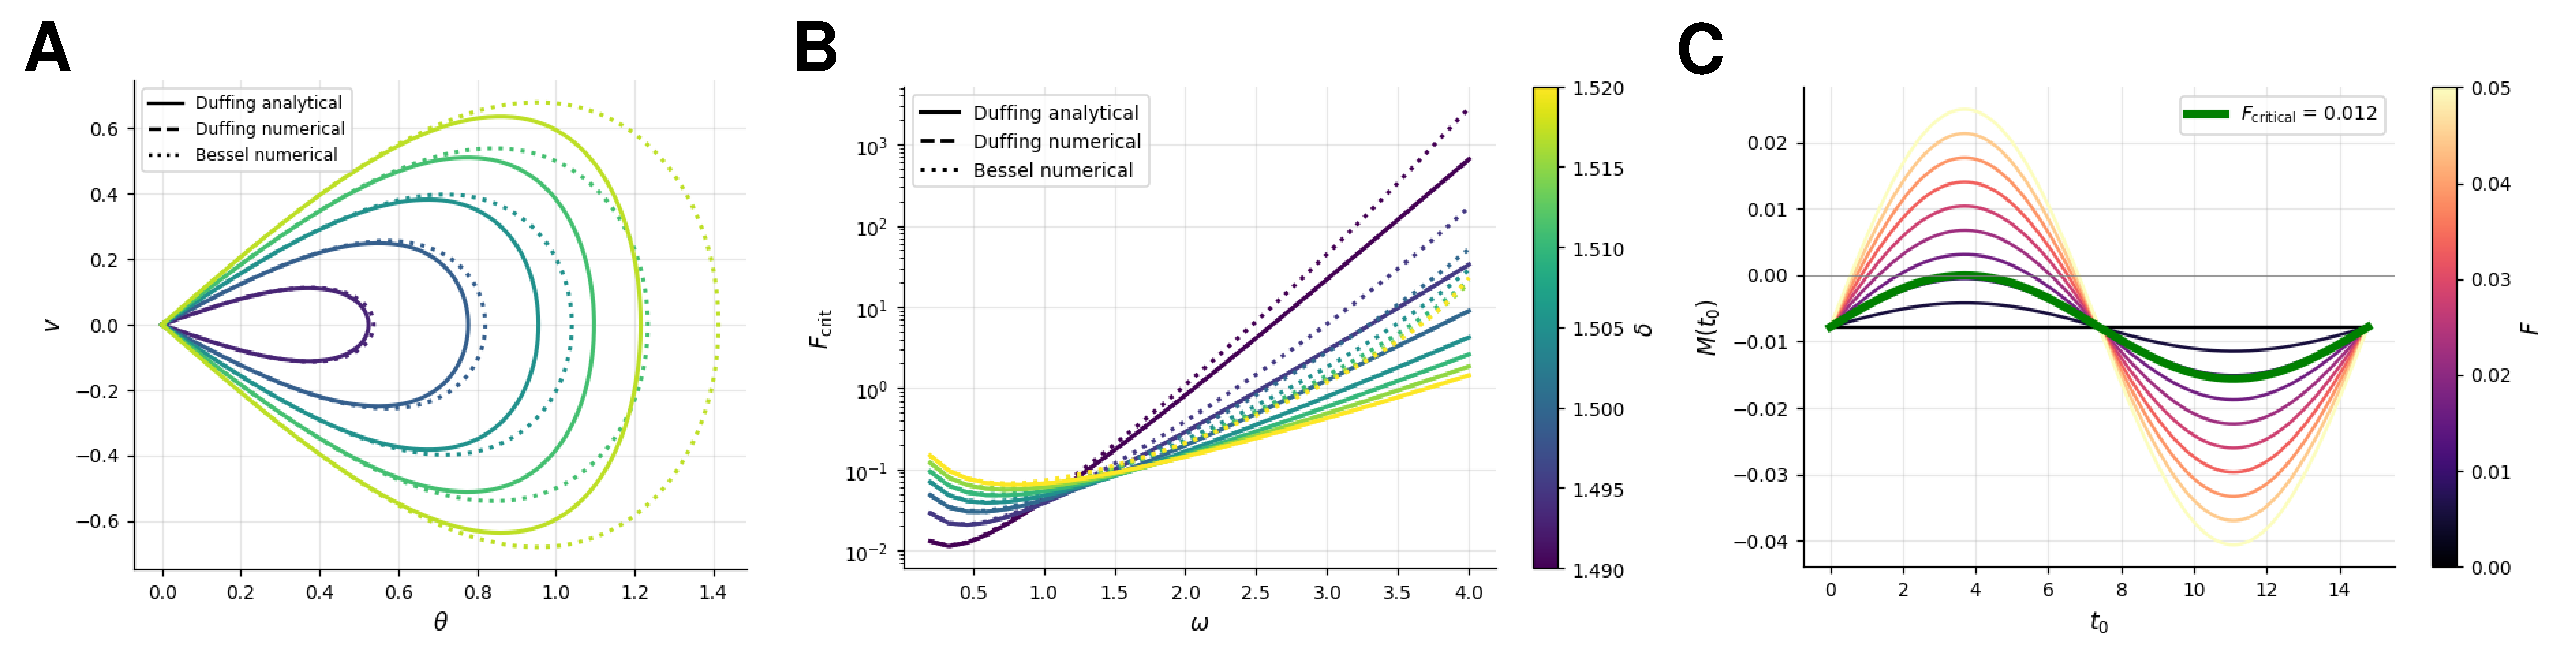
\includegraphics[width=\textwidth]{figures/fig4.pdf}
  \caption{Melnikov analysis comparing the Duffing and Bessel homoclinics.  (A)
  Phase-plane overlay of the three homoclinic orbits across $\delta \in [1.49,
  1.52]$.  (B) $F_{\mathrm{crit}}(\omega)$ on a log scale; the Bessel curve
  (dotted) peels above the Duffing at high $\omega$.  (C) Melnikov function
  $M(t_0)$ vs.\ $t_0$ for $F$ swept from $0$ to $0.05$; bold green curve marks
  $F = F_{\mathrm{crit}}$.}
  \label{fig:melnikov}
\end{figure}


% ─────────────────────────────────────────────────────────────────────────────
\subsection{Numerical Verification Near the Homoclinic-Resonance Frequency}
\label{sec:numerical-verification}
% ─────────────────────────────────────────────────────────────────────────────

We perform a grid search over the forcing amplitude.  With the chosen parameters,
\cref{eq:Fcrit} gives $F_{\mathrm{crit}} \approx 0.012$, and we grid
%
\begin{equation}
\label{eq:F-grid}
F \in \{1.0,\; 1.5,\; 2.0,\; 2.5,\; 3.0\} \times F_{\mathrm{crit}},
\end{equation}
%
integrating \cref{eq:duffing-unforced} for the reduced Duffing model and the
12-neuron discrete circuit from initial conditions in the right well
($\theta_0 = \sqrt{A/B}$, $v_0 = 0$).  We verified numerically (not shown) that
the 12-neuron model yields an empirically very similar $U(\theta)$ and comparable
behaviour under perturbation to the Bessel limit.  For each run we discard the
first 200 forcing periods as transient and record the next 1000 stroboscopic
samples $(\theta_n, v_n)$ at $t_n = 2\pi n/\omega$.  We then sweep $F$ over a
denser grid to construct the Poincaré bifurcation diagram $\theta_n$ vs.\ $F$.

\Cref{fig:poincare} presents three rows: (A) reduced Duffing, (B) 12-neuron full
circuit at $\delta = 1.49$ (bistable regime), and (C) 6-neuron full circuit at
the same parameters, which --- as previously shown --- possesses only a single
attractor (monostable regime).  Each row contains four panels: (i) stroboscopic
Poincaré sections at the five grid-search values of $F$; (ii) Poincaré
bifurcation diagram on a narrow zoom $F \in [0, 0.1]$ revealing the route to
chaos; (iii) full phase-space trajectories at the five $F$ values; (iv)
bifurcation diagram on a wide zoom $F \in [0, 10]$ exposing the large-forcing
regime studied in \cref{sec:phase-slipping}.

Across both the reduced Duffing (row A) and the 12-neuron circuit (row B), we
observe the same qualitative structure.  At $F = F_{\mathrm{crit}}$ the attractor
is a period-1 orbit confined to the right well.  By $F \approx
1.5\,F_{\mathrm{crit}}$ the periodic orbit has lost stability and the trajectory
fills a strange attractor exploring both wells.  The bifurcation diagrams in
panel (ii) show characteristic interleaving of chaotic bands and narrow periodic
windows.  By $F \approx 2.5$--$3\,F_{\mathrm{crit}}$ the trajectory recollects
onto a large-amplitude periodic orbit encircling both centres.

The factor-of-1.5 gap between the Melnikov threshold and the visible onset of
chaos may reflect that the Melnikov threshold proves existence of the horseshoe
but does not determine whether the invariant set is an attractor.  Nonetheless,
the quantitative agreement between the reduced model (A) and the 12-neuron
circuit (B) validates the Duffing reduction as a faithful predictor of chaos
onset in the biological circuit.

Row (C) provides a control: in the monostable regime, the unforced system has a
single stable fixed point and no homoclinic orbit.  Correspondingly, the
trajectories in panel (C-iii) remain periodic across the entire grid.  The
strange attractor of rows (A) and (B) is therefore a direct consequence of the
double-well structure produced by the pitchfork bifurcation.

\begin{figure}[htbp]
  \centering
  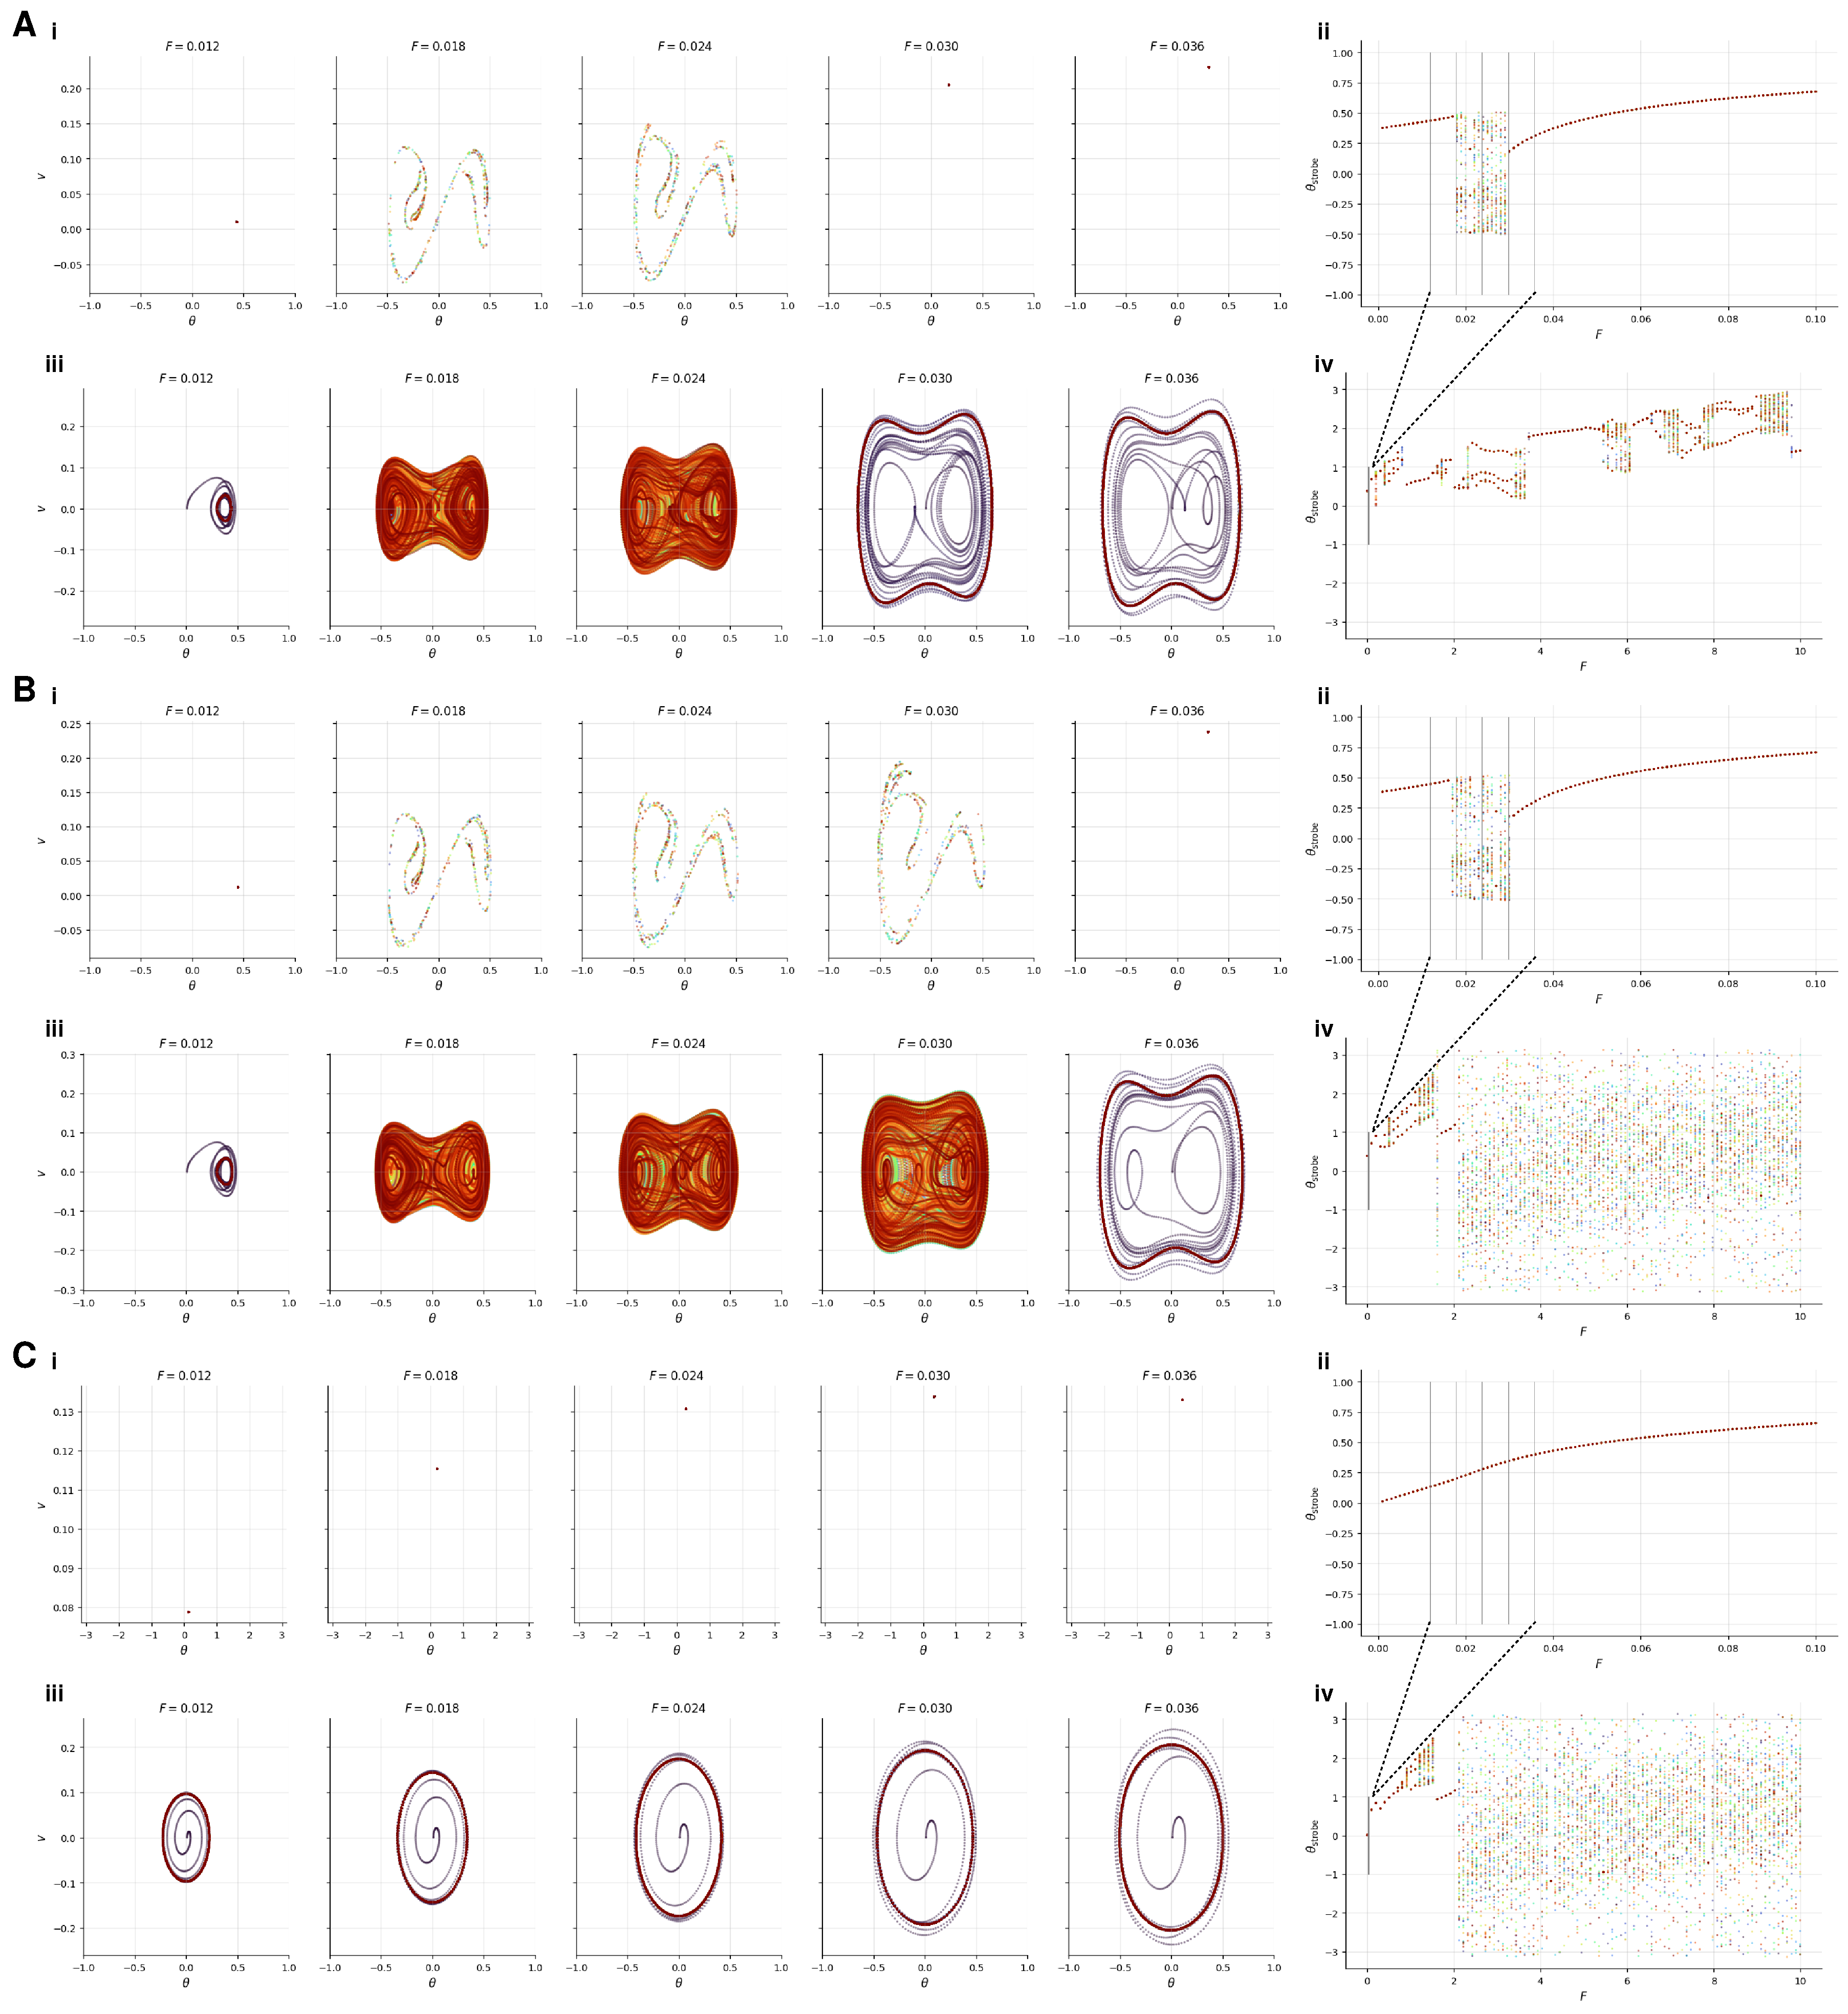
\includegraphics[width=\textwidth]{figures/fig5.pdf}
  \caption{Poincaré sections, bifurcation diagrams, and phase-space trajectories
  for (A) the reduced Duffing model, (B) the 12-neuron circuit in the bistable
  regime ($\delta = 1.49$), and (C) the 6-neuron circuit in the monostable
  regime.  Each row contains panels (i) stroboscopic Poincaré sections at five
  forcing amplitudes; (ii) narrow-zoom Poincaré bifurcation diagram; (iii)
  phase-space trajectories; (iv) wide-zoom bifurcation diagram.}
  \label{fig:poincare}
\end{figure}


% ─────────────────────────────────────────────────────────────────────────────
\subsection{A Second Chaotic Regime: Phase Slipping and the Pendulum Analogy}
\label{sec:phase-slipping}
% ─────────────────────────────────────────────────────────────────────────────

The wide-zoom bifurcation diagrams in panels (A-iv) and (B-iv) of
\cref{fig:poincare}, together with the snapshots in \cref{fig:phaseslip}, reveal
a striking divergence between the reduced and full systems at large forcing
amplitudes ($F \gtrsim 2$, two orders of magnitude above $F_{\mathrm{crit}}$).

In the reduced Duffing model (\cref{fig:phaseslip}A), increasing $F$ eventually
drives the trajectory out of the chaotic regime into a large-amplitude periodic
orbit encircling both wells.  The Poincaré section consists of isolated points
and the phase-space trajectory is a smooth closed curve oscillating between
$\theta \approx \pm 3$ --- the familiar global periodic attractor of the
standard forced Duffing oscillator.

The full circuit (\cref{fig:phaseslip}B) behaves qualitatively differently in
the same parameter range.  Rather than settling onto a closed periodic orbit,
the trajectory undergoes \textbf{phase slipping}: $\theta$ executes net rotations around
the cylinder $S^1$ rather than remaining bounded.  The Poincaré sections are
wide diffuse clouds extending across the full range of $\theta$ and reaching
velocities $|v| \sim 10$, an order of magnitude larger than in the Duffing-type
chaos of \cref{fig:poincare}.

This phenomenon is invisible to the Duffing reduction, but is naturally
understood through analogy with the forced damped pendulum,
%
\begin{equation}
\label{eq:pendulum}
\ddot\varphi + \gamma\dot\varphi + \sin\varphi = F\cos\omega t,
\end{equation}
%
which has been studied extensively as a model system for chaos on the phase
cylinder \cite{guckenheimer1983}.  The pendulum has two equivalent saddle points
at $\varphi = \pm\pi$ (identified on $S^1$) connected by two heteroclinic orbits
--- the upper and lower branches of the separatrix bounding librating versus
rotating motion.  Under periodic forcing, transverse intersections of the stable
and unstable manifolds of these heteroclinic connections generate a chaotic
invariant set on which the trajectory irregularly switches between librating and
rotating behaviour.

Our full Bessel system inherits this pendulum-like structure: the steering drive
$U(\theta, \delta)$ vanishes at $\theta = 0$ (the unstable saddle between the
two goals) and at $\theta = \pm\pi$ (the saddles at the anti-midpoint; cf.\
\cref{fig:bifurcation}, right panel).  When the trajectory has enough energy to
traverse the global separatrix, it can transit between adjacent saddles,
producing phase slipping analogous to the rotating regime of the forced pendulum.
The chaotic dynamics of \cref{fig:phaseslip}B is most naturally attributed to
transverse intersection of the heteroclinic manifolds connecting the $\theta =
\pm\pi$ saddles.

A direct comparison is provided by row C of \cref{fig:phaseslip}, which applies
the same large-$F$ protocol to the monostable regime of \cref{fig:poincare}C.
In this configuration the cubic reduction predicts no chaos at any $F$ --- there
is no double-well structure and no homoclinic orbit.  Yet the full system
(\cref{fig:phaseslip}C) still exhibits phase-slipping chaos at large $F$,
qualitatively indistinguishable from \cref{fig:phaseslip}B.  This is direct
evidence that the second chaotic regime is not a consequence of the goal-induced
double well but of the global $S^1$ topology of the steering drive.  The reduced
Duffing model is silent on this regime precisely because the cubic truncation
captures the saddle at $\theta = 0$ but discards the saddles at $\theta = \pm\pi$.

A Melnikov analysis of phase-slipping chaos is conceptually straightforward but
operationally involved; the resulting chaos threshold would depend on $(\delta,
\kappa, \gamma, \omega)$ through circuit-specific integrals analogous to
\cref{eq:D-integral}.  We leave this as a direction for future work.  For the
present, we record the numerical demonstration that two distinct chaotic regimes
exist in the steering circuit --- one captured faithfully by the Duffing
reduction near $F_{\mathrm{crit}}$, and a second, global regime accessible only
through the full Bessel or neural circuit model.

\begin{figure}[htbp]
  \centering
  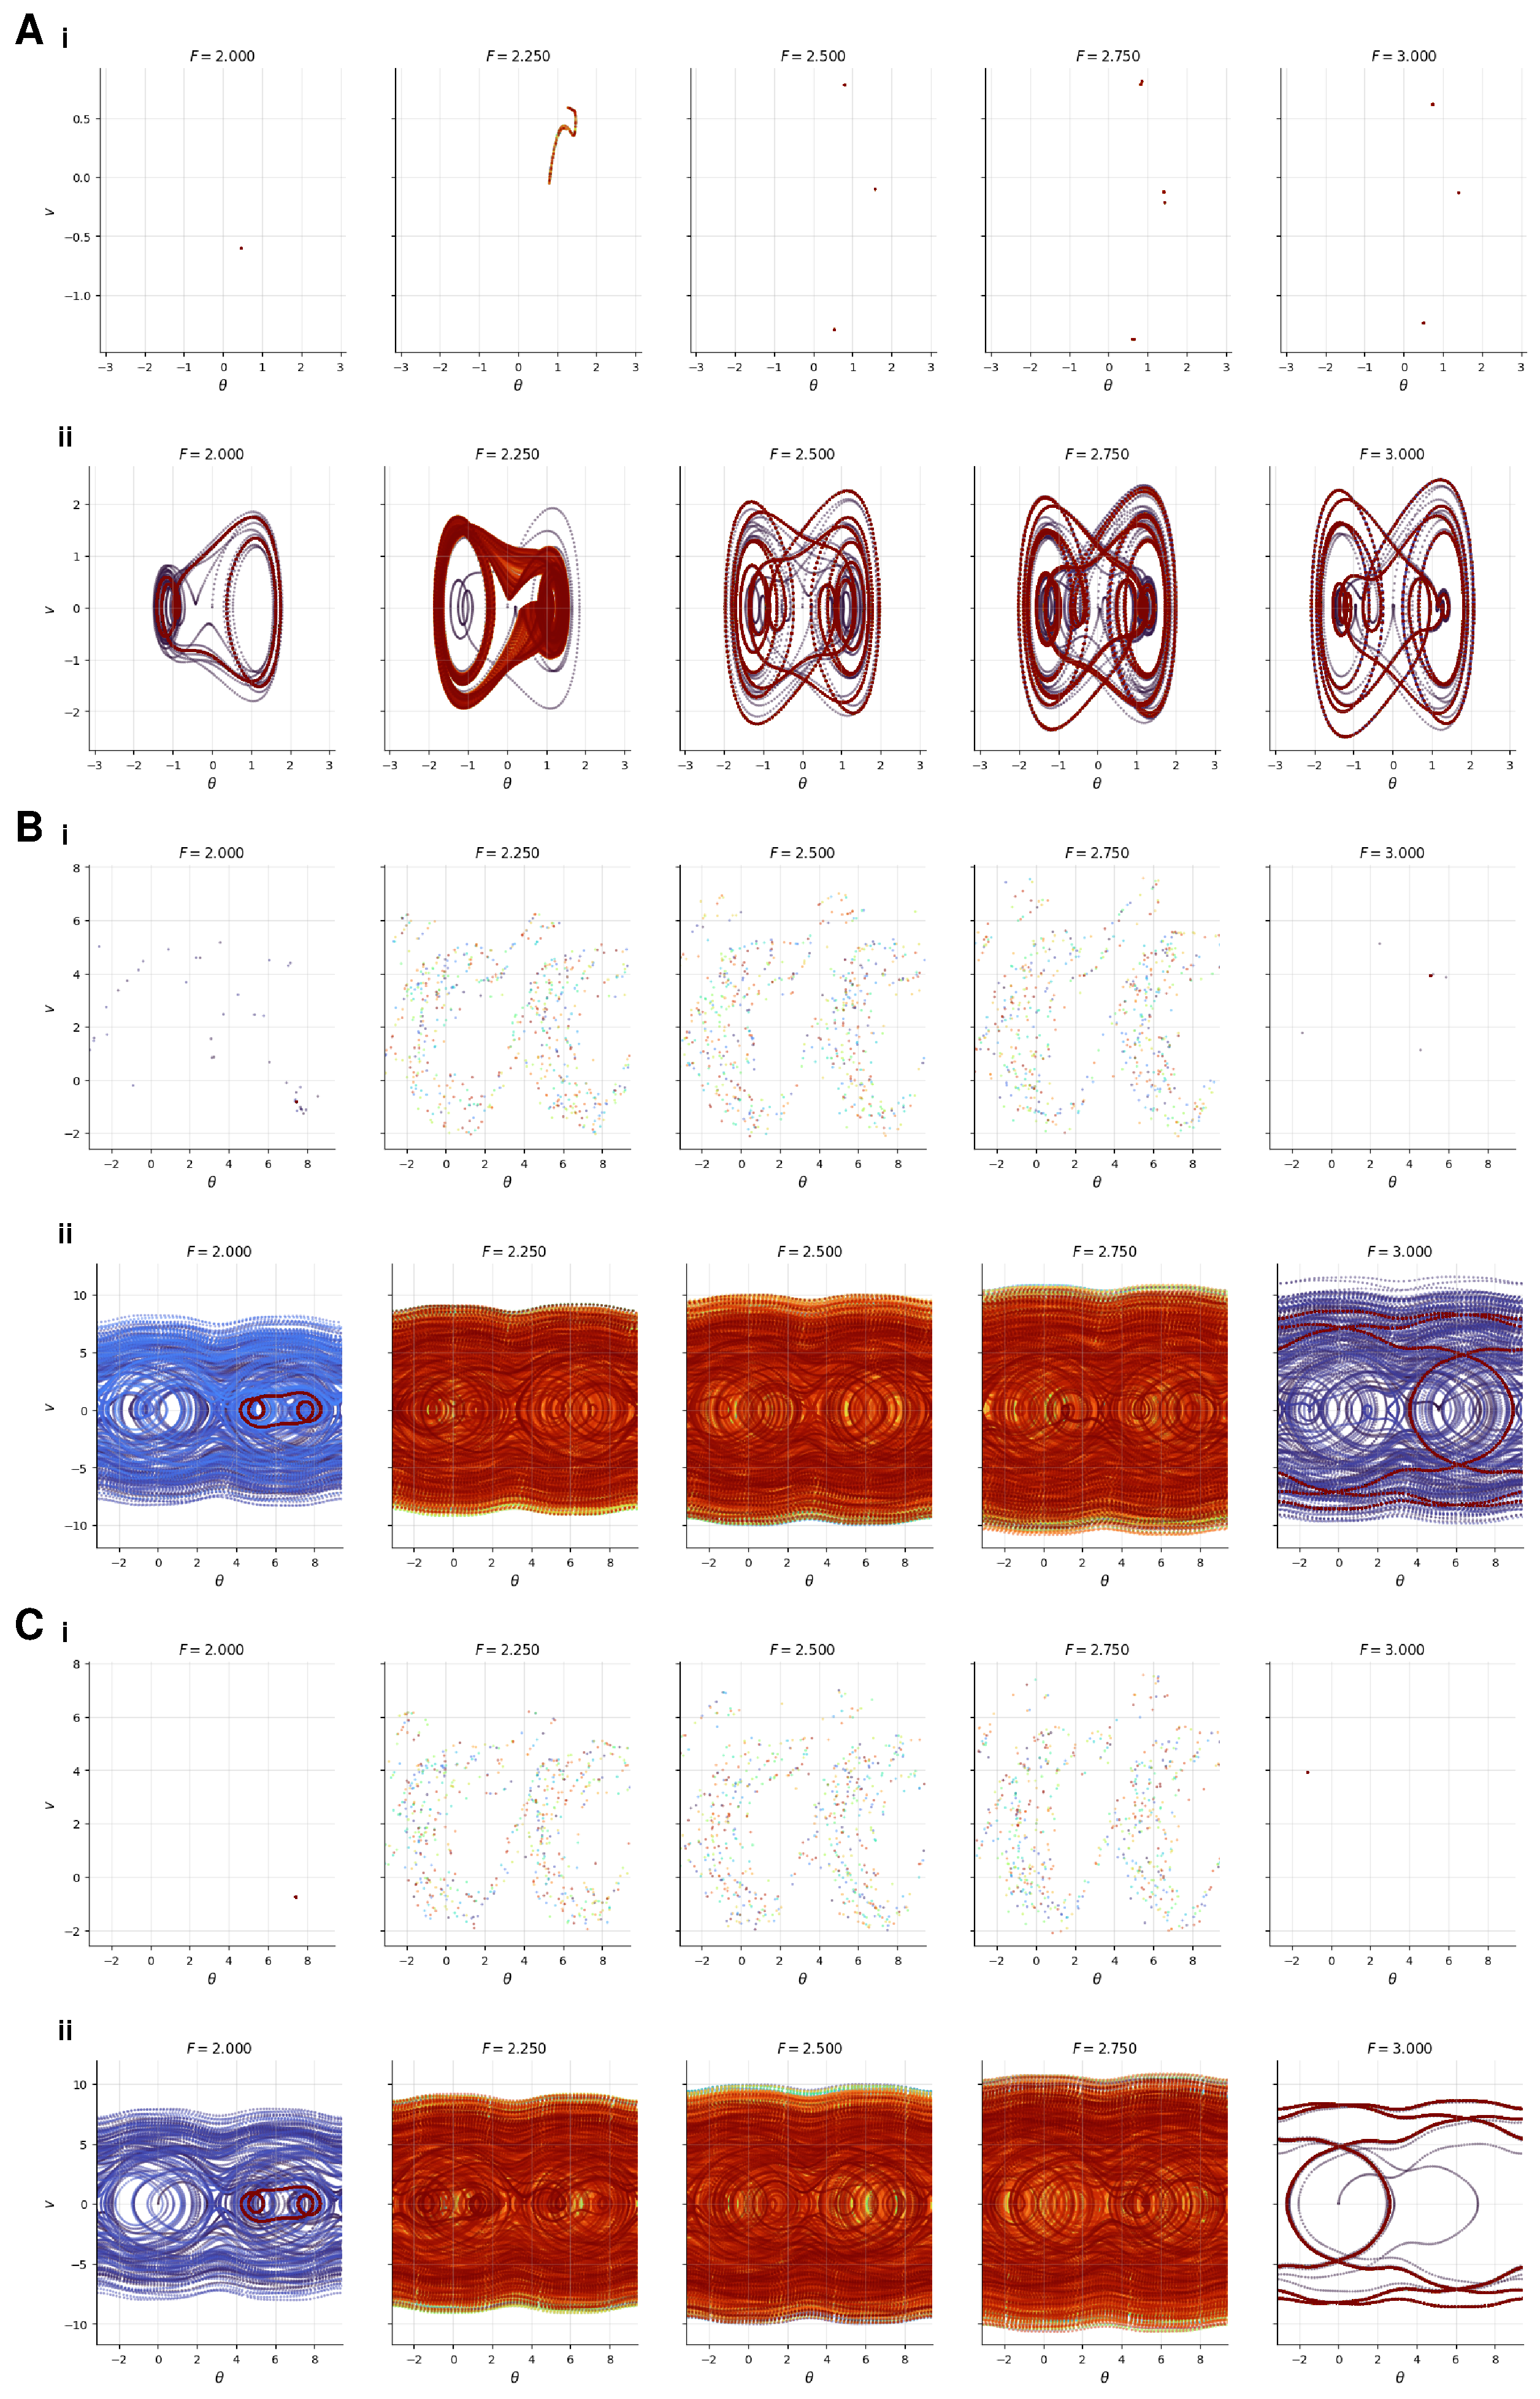
\includegraphics[width=0.8\textwidth]{figures/fig6.pdf}
  \caption{Large-amplitude forcing regime for (A) the reduced Duffing model,
  (B) the full circuit in the bistable regime, and (C) the full circuit in the
  monostable regime.  Each case shows (i) Poincaré sections and (ii) phase-space
  trajectories.  Rows B and C both exhibit phase-slipping chaos absent from the
  Duffing reduction.}
  \label{fig:phaseslip}
\end{figure}


% ─────────────────────────────────────────────────────────────────────────────
\section{Discussion}
\label{sec:discussion}
% ─────────────────────────────────────────────────────────────────────────────

Our analysis has established that the \textit{Drosophila} steering circuit,
under the assumption of dual-goal von Mises representations, generates a local
cubic normal form whose forced version supports two distinct chaotic regimes: a
local, goal-induced homoclinic chaos near the Melnikov threshold, and a global,
pendulum-like heteroclinic chaos at larger forcing.  Whether either regime is
realised in the behaving fly, and which natural perturbations could induce them,
depend on several factors that this work does not fully resolve.  We close by
outlining what is needed to bridge the theoretical analysis to biological
validation.

% ─────────────────────────────────────────────────────────────────────────────
\subsection{Inertia, Friction, and the Realised \texorpdfstring{$F(\omega)$}{F(omega)} Surface}
\label{sec:inertia}
% ─────────────────────────────────────────────────────────────────────────────

The Melnikov criterion \eqref{eq:Fcrit} gives $F_{\mathrm{crit}}$ as a function
of the dimensionless parameters $A, B, \gamma, \omega$, but the mapping back to
physical forcing amplitudes and frequencies depends sensitively on the body's
rotational inertia $I$ and frictional drag $\gamma_{\mathrm{phys}}$.  In our
units (setting $I = 1$, which rescales time by $\sqrt{I/T_0}$ with $T_0$ a
reference torque), the dimensionless $\omega$ corresponds to a physical frequency
$\omega_{\mathrm{phys}} = \omega\sqrt{T_0/I}$.  The dual-goal chaos predicted
near $F_{\mathrm{crit}} \sim 0.01$ in our units may correspond to physical torque
perturbations within or beyond the range deliverable by natural sensory streams,
depending on these calibration factors.

This caveat applies most stringently to the local chaos of \cref{sec:numerical-verification},
which occupies a narrow window in $(F, \omega)$: the homoclinic resonance is
sharp, and a mismatch between the natural frequencies of biological perturbations
and the system's $\omega \approx 0.76\sqrt{A}$ may suppress visible chaos.  The
phase-slipping chaos of \cref{sec:phase-slipping}, by contrast, persists across
two orders of magnitude in $F$ and is more robust to the choice of frequency.
If the goal is to observe chaotic steering experimentally --- for instance, via
optogenetic perturbations or visual stimulation at a chosen frequency --- the
phase-slipping regime is more accessible, requiring only that the forcing
amplitude be large enough to push the system into the rotational regime of the
phase cylinder.

% ─────────────────────────────────────────────────────────────────────────────
\subsection{The Melnikov Bound is Approximate}
\label{sec:melnikov-approx}
% ─────────────────────────────────────────────────────────────────────────────

The factor of approximately $1.5$ between the Melnikov threshold and the
observable onset of chaos in \cref{sec:numerical-verification} may be attributed
to two sources.  First, the Melnikov function is leading-order in the
perturbation parameter $\epsilon$, which may deviate from the true threshold to
the horseshoe by $O(\epsilon^2)$.  Second, the horseshoe born at the Melnikov
threshold is not necessarily an attractor, so its existence does not by itself
imply observable chaos.  We did not run dedicated numerical experiments to
disentangle these two contributions.

Empirically, the gap is likely a complicated function of $\omega$.  At high
$\omega$, $F_{\mathrm{crit}}$ grows exponentially through the $\cosh$ factor and
the perturbation parameter $F/\sqrt{2A^3/B}$ leaves the small-$\epsilon$ regime
entirely, so \cref{eq:Fcrit} ceases to be reliable as a quantitative predictor.
Mapping this gap numerically across the $(\omega, \delta)$ plane is a natural
next step before attempting to predict experimental chaos-onset parameters.

Further, the deterministic forced Duffing analysis presented here neglects
stochasticity, which is unrealistic in biological systems.  We leave further
explorations of stochastic effects to future work.

% ─────────────────────────────────────────────────────────────────────────────
\subsection{Representation of Dual Goals}
\label{sec:dual-goal-rep}
% ─────────────────────────────────────────────────────────────────────────────

Our entire analysis rests on the representation of two simultaneous goals as a
superposition of two von Mises bumps with equal amplitude and concentration.
Biologically, the goal representation could also be implemented as temporal
switching between two single-goal bumps (winner-takes-all dynamics with
stochastic transitions), or as a deformed single bump shifted toward the
resultant direction.  The von Mises superposition is the only one of these
representations that genuinely yields bistability in the steering drive: as
established in \cref{sec:intro}, single-bump representations collapse to
unimodal steering profiles and cannot generate a pitchfork bifurcation.  The
phase-slipping chaos of \cref{sec:phase-slipping}, however, is independent of
the dual-goal structure and would persist under any representational scheme,
since it arises from the global $S^1$ topology of the steering drive rather than
from the goal-induced double well.

% ─────────────────────────────────────────────────────────────────────────────
\subsection{The Role of PFL2 and the Nonlinearity Choice}
\label{sec:pfl2}
% ─────────────────────────────────────────────────────────────────────────────

It is worth noting that the full circuit model (with PFL2 cells and the indirect
pathway) yields surprisingly similar $U(\theta)$ profiles to the PFL3-only
reduction (\cref{fig:U-profiles}), suggesting a redundancy of PFL2 in our model
that contradicts experimental observations of PFL2's role
\cite{westeinde2024}.  This inconsistency may result from our choice of quadratic
nonlinearity $f(x) = x^2$ rather than the ELU used in Westeinde et al.\
\cite{westeinde2024}.  The ELU's asymmetric rectification could act as a gating
mechanism, selectively activating subpopulations of control neurons in a manner
that the quadratic model cannot capture.  A more rigorous analysis of the
complete circuit model, including more biologically informed nonlinearity choices,
would clarify whether PFL2 plays a structural role in shaping the chaos
thresholds of the steering system.  Combined with the switching-bump
representations discussed in \cref{sec:dual-goal-rep}, this would form a fuller
theoretical picture of how the central complex's neural architecture supports
robust multi-goal navigation in the face of perturbations.


% ─────────────────────────────────────────────────────────────────────────────
\section*{Notation and Conventions}
\label{sec:notation}
% ─────────────────────────────────────────────────────────────────────────────
\addcontentsline{toc}{section}{Notation and Conventions}

For ease of cross-reference:
\begin{itemize}
  \item $\theta$: fly's heading.
  \item $\delta$: half-separation of the two goals (goals at $\pm\delta$).
  \item $\phi$: preferred direction of a PFL/goal/heading neuron (integration variable).
  \item $\Dp$: PFL3L heading-input phase shift ($+67.5°$ for L, $-67.5°$ for R).
  \item $\kh,\, \kg$: von Mises concentrations of heading and goal bumps; often taken equal to $\kappa$.
  \item $\kappa(a, b) = \sqrt{\kh^2 + \kg^2 + 2\kh\kg\cos(a-b)}$: effective concentration after phasor sum.
  \item $\mu(a, b)$: effective phase; drops out after integration over $\phi$.
  \item $S, A$: synaptic gain on heading and goal inputs (both positive; set by biology).
  \item $f(x) = x^2$: quadratic nonlinearity (conjunctive tuning).
  \item $U(\theta, \delta) = G_{\mathrm{PFL3L}} - G_{\mathrm{PFL3R}}$: total steering drive.
\end{itemize}


% ─────────────────────────────────────────────────────────────────────────────
\printbibliography
% ─────────────────────────────────────────────────────────────────────────────

\end{document}
